\section{Auswertung} 

\subsection{Wheatstonesche Brücke}
\begin{flushleft}
    Der Unbekannte $R_{x}$ wird mit der Hilfe der Formel (\ref{4}) berechnet. 
\end{flushleft}

\begin{table}[H]
    \centering
    \caption{Die Messwerte der Wheatstoneschen Brücke mit dem $R_{x}$ für Wert 10. }
    \label{Tabelle1}
    \begin{tabular} {c  c  c  c}
        \toprule
        {$ $} &
        {$ \text{Messung 1} $} &
        {$ \text{Messung 2} $} &
        {$ \text{Messung 3} $} \\
        \midrule
        $R_{x}$ & 237,46\,\unit{\ohm} & 229,81\,\unit{\ohm} & 238,44\,\unit{\ohm}  \\
        $R_{2}$ & 500\,\unit{\ohm}    & 644\,\unit{\ohm}    & 332\,\unit{\ohm}     \\
        $R_{3}$ & 322\,\unit{\ohm}    & 263\,\unit{\ohm}    & 418\,\unit{\ohm}     \\
        $R_{4}$ & 678\,\unit{\ohm}    & 737\,\unit{\ohm}    & 582\,\unit{\ohm}     \\
        \bottomrule
    \end{tabular} 
\end{table}

\begin{align*}
    \intertext{Der Wert $R_{x}$ wird gemittelt und die dazugehörige Abweichung berechnet}
    R_{\text{x,Wert 10}} = (235,24 \pm 4,72)\,\unit{\ohm}.
\end{align*}

\begin{table}[H]
    \centering
    \caption{Die Messwerte der Wheatstoneschen Brücke mit dem $R_{x}$ für Wert 13. }
    \label{Tabelle2}
    \begin{tabular} {c  c  c  c}
        \toprule
        {$ $} &
        {$ \text{Messung 1} $} &
        {$ \text{Messung 2} $} &
        {$ \text{Messung 3} $} \\
        \midrule
        $R_{x}$ & 318,98\,\unit{\ohm} & 318,33\,\unit{\ohm} & 316,790\,\unit{\ohm}  \\
        $R_{2}$ & 332\,\unit{\ohm}    & 500\,\unit{\ohm}    & 644\,\unit{\ohm}     \\
        $R_{3}$ & 490\,\unit{\ohm}    & 389\,\unit{\ohm}    & 323\,\unit{\ohm}     \\
        $R_{4}$ & 510\,\unit{\ohm}    & 611\,\unit{\ohm}    & 677\,\unit{\ohm}     \\
        \bottomrule
    \end{tabular} 
\end{table}

\begin{align*}
    \intertext{Daraus folgt}
    R_{\text{x,Wert 13}} = (318,03 \pm 1,12)\,\unit{\ohm}.
\end{align*}


\subsection{Kapazitätmessbrücke}

\begin{align*}
    \intertext{Die Berechnung der Werte $C_{x}$ und $R_{x}$ folgt nach den Formeln (\ref{4}) und (\ref{5}). }
\end{align*}

\begin{table}[H]
    \centering
    \caption{Die Messwerte der Kapazitätsmessbrücke mit dem $R_{x}$ für Wert 15 und Wert 11.}
    \label{Tabelle3}
    \begin{tabular} {c  c  c  c}
        \toprule
        {$ $} &
        {$ \text{Messung 1} $} &
        {$ \text{Messung 2} $}\\
        \midrule
        $C_{2}$ & 399\,\unit{\nano\farad} & 399\,\unit{\nano\farad} \\
        $R_{2}$ & 805\,\unit{\ohm} & 0\,\unit{\ohm}   \\
        $R_{3}$ & 359\,\unit{\ohm} & 376\,\unit{\ohm} \\
        $R_{4}$ & 611\,\unit{\ohm} & 624\,\unit{\ohm} \\
        $C_{x}$ & 626\,\unit{\nano\farad} & 662\,\unit{\nano\farad} \\
        $R_{x}$ & 512\,\unit{\ohm} & 0\,\unit{\ohm}   \\
        \bottomrule
    \end{tabular} 
\end{table}

\begin{align*}
    \intertext{Die Berechnung wird gemittelt und die Standardabweichung gebildet.}
    C_{\text{x,Wert 15}} = (644 \pm 25,45)\,\unit{\nano\farad}.
\end{align*}

\subsection{Induktivitätsbrücke}

\begin{align*}
    \intertext{Mit Hilfe der Formeln (\ref{6}) und (\ref{4}), sowie mit einer eingestellten Frequenz von $v = 1076\,\unit{\hertz}$, ergiben sich folgende Werte. }
\end{align*}

\begin{table}[H]
    \centering
    \caption{Die Messwerte der Induktivitätsmessbrücke mit dem $L_{x}$ und $R_{x}$ für den Wert 18.}
    \label{Tabelle4}
    \begin{tabular} {c  c}
        \toprule
        {$ $} &
        {$ \text{Messung 1} $} \\
        \midrule
        $L_{2}$ & 14,6\,\unit{\milli\henry}\\
        $R_{2}$ & 90\,\unit{\ohm} \\
        $R_{3}$ & 820\,\unit{\ohm} \\
        $R_{4}$ & 180\,\unit{\ohm} \\
        $L_{x}$ & 66,5\,\unit{\milli\henry}\\
        $R_{x}$ & 410\,\unit{\ohm} \\
        \bottomrule
    \end{tabular} 
\end{table}

\subsection{Maxwell-Brücke}

\begin{align*}
    \intertext{Die Messwerte $L_{x}$ und $R_{x}$ ergeben sich über die Formeln (\ref{7}) und (\ref{8}).}
\end{align*}

\begin{table}[H] 
    \centering
    \caption{Die Messwerte der Maxwell-Brücke mit $L_{x}$ und $R_{x}$ für den Wert 18.}
    \label{Tabelle5}
    \begin{tabular} {c  c}
        \toprule
        {$ $} &
        {$ \text{Messung 1} $} \\
        \midrule
        $R_{2}$ & 664\,\unit{\ohm} \\
        $R_{3}$ & 205\,\unit{\ohm} \\
        $R_{4}$ & 420\,\unit{\ohm} \\
        $C_{4}$ & 399\,\unit{\nano\farad}\\
        $L_{x}$ & 54,3\,\unit{\milli\henry}\\
        $R_{x}$ & 324\,\unit{\ohm} \\
        \bottomrule
    \end{tabular} 
\end{table}

\subsection{Wien-Robinson-Brücke}


\begin{align*}
    \intertext{Die Frequenzabhängigkeit der Brückenspannung wird im Bereich $ 20\,\unit{\hertz} \leq v \leq 30000\,\unit{\hertz} $ untersucht. Dazu wird der Quotient $\frac{U_{\text{Br}}}{U_{\text{S}}}$ 
    gegen $\unit{\ohm} = \frac{v}{v_{0}}$ in einem halbalgortihmischen Diagramm aufgetragen.}
    \intertext{Ab welcher Frequenz die Brückenspannung verschwinden sollte, wird nach den folgenden Formeln berechnet:}
    \omega_{0} = \frac{1}{RC} = \frac{1}{1000\,\unit{\ohm} \cdot 660\,\unit{\nano\farad}} = 1515,15\,\unit{\hertz} \\
    v_{0} = \frac{\omega_{0}}{2\pi} = \frac{1}{2\pi RC} = 241,14\,\unit{\hertz}.\\
\end{align*}



\begin{table}[H] 
    \centering
    \caption{Die Messwerte der frequenzabhängigen Spannung.}
    \label{Tabelle6}
    \begin{tabular} {c  c}
        \toprule
        {$ v \mathbin{/} \unit{\hertz} $} &
        {$ U_{\text{Br}} \mathbin{/} \unit{\volt} $} \\
        20    & 3,20  \\
        50    & 2,80  \\
        100   & 1,98  \\
        150   & 1,10  \\
        200   & 0,44  \\
        220   & 0,20  \\
        230   & 0,10  \\
        240   & 0,017 \\
        250   & 0,085 \\
        260   & 0,17  \\
        280   & 0,34  \\
        300   & 0,48  \\
        400   & 1,15  \\
        500   & 1,60  \\
        750   & 2,30  \\
        1000  & 2,60  \\
        2000  & 3,10  \\
        5000  & 3,20  \\
        10000 & 3,05  \\
        15000 & 2,80  \\
        20000 & 2,30  \\
        \midrule
        \bottomrule
    \end{tabular} 
\end{table}


\begin{figure}[H]
    \centering
    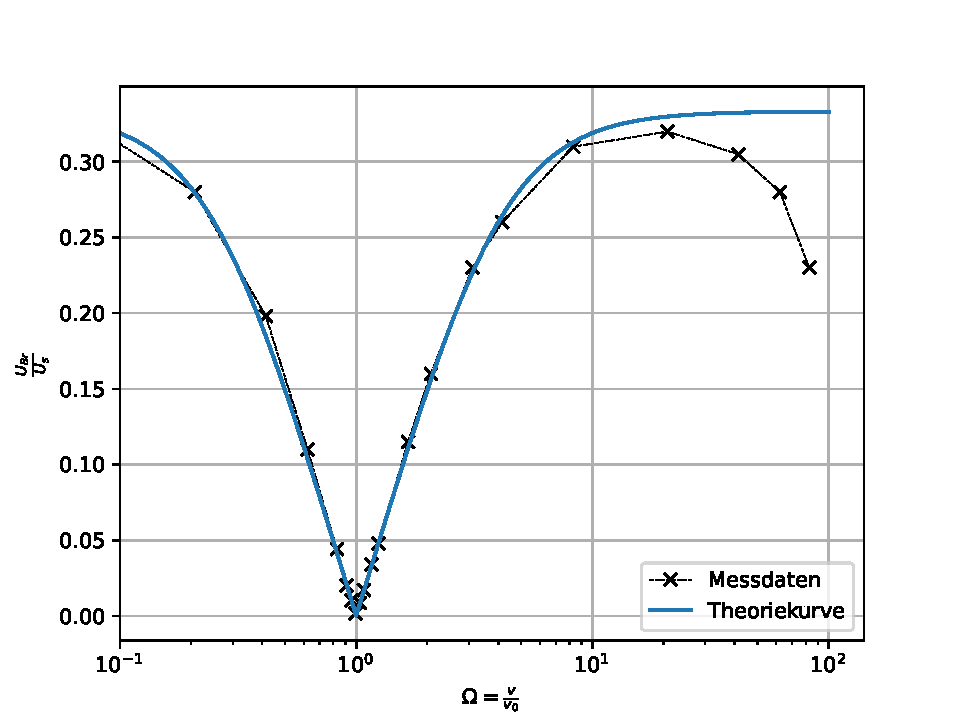
\includegraphics[height=100mm]{bilder/plot2.pdf}
    \caption{Die graphische Darstellung der Messwerte für die frequenzabhängige Spannung mit der Ausgleichsfunktion.\label{Abbildung9} }
\end{figure}

\begin{flushleft}
    Wie an der Kurve zu erkennen, verschwindet die Brückenspannung bei ungefähr $V_{0} = 240\,\unit{\hertz}$. 
    Für die Bestimmung des Klirrfaktors wird die Formel (\ref{11}) benutzt. 
    Wie zu erkennen, benötigt man den Wert $U_{2}$, welcher aus (\ref{10}) errechnet werden kann. 
    Dabei ist $U_{1} = 10\,\unit{\volt}$ aus $U_{\text{S}}$. 
    Daraus folgt mit $\unit{\ohm} = 2$:
\end{flushleft}

\begin{align*}
    U_{2} = \frac{0,004\unit{\volt}}{ \sqrt{\frac{(2^2 -1)^2}{9(1-2^2)^2 + 9 \cdot 2^2}}} = 0,01442\,\unit{\volt}.
    \intertext{Anschließend folgt für den Klirrfaktor}
    k = \frac{U_{2}}{U_{1}} = 1,442 \cdot 10^{-3}.
\end{align*}

\newpage